\chapter{In-depth analysis phase}
\label{chap:indepthreport}
\section{Organisational setup}
DANX is founded by Søren Gønge and now co-owned by Bob Thorhauge.\cite{malene002}\\
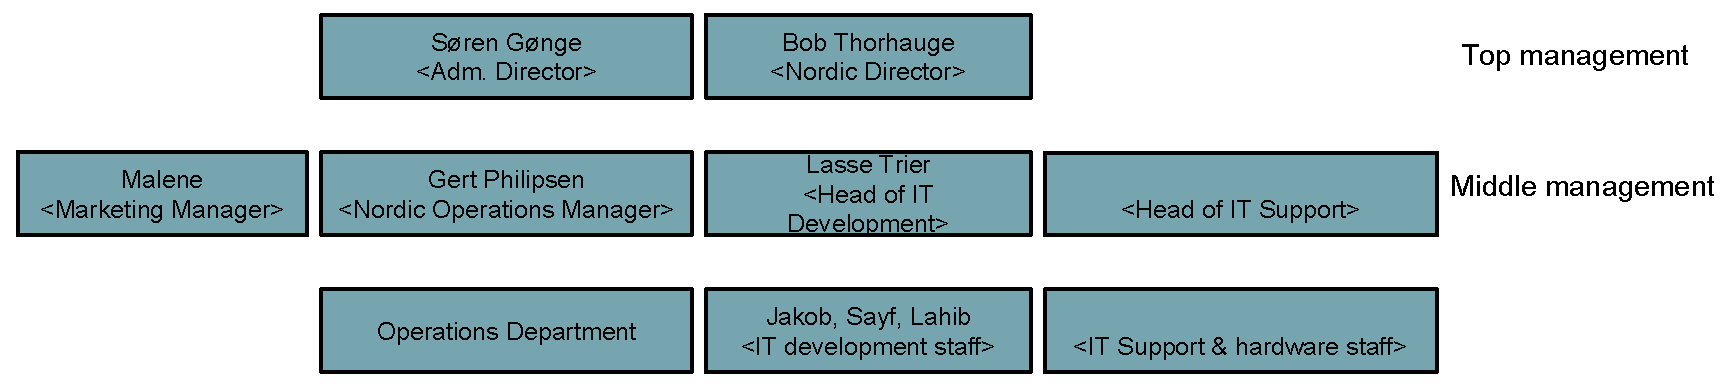
\includegraphics[scale=0.55]{img/Organizational_Chart}

\section{Key players}
This section describes the persons that have the most significant impact on the project.

\subsection{Lasse Trier}
Lasse Trier is the head of IT development. His main responsibility is to integrate customer’s IT systems and provide customer support when complications occur.\cite{lahib003}\cite{lahib004}\\
Additionally he prioritizes and delegates the tasks of three other employees of the development department.\cite{lasse009} He has an important role in providing competitive advantages to DANX as described in the Strategic Alignment Report in Work Domains. His impact on the project is significant, because he provides solutions to customer problems.

\subsection{Gert Philipsen}
Gert Philipsen is the head of the operational department. His responsibility is ensuring that DANX delivers on-time by coordinating and leading the operational department. He is concerned, among other things, with optimization of the operational department\cite{gert015}, which makes his opinion on the project important.

\section{Current work practices}
\label{sec:workpractices}
This section describes the work practices of the operational, IT development and IT support department that are relevant to the problem. The control tower is part of the operational department.\\
When customers of DANX wants to report a problem to DANX, they contact the control tower in the majority of cases.\cite{gert004} Customers can contact employees on other levels than the employees of the control tower.\cite{gert007} Customers can contact danx through phone or email, but mostly uses email.\cite{gert020} Each employee providing customer support has his own computer.\cite{gert024} The employee that receives the request might be able to solve the problem, if not, it is propagated.\\
The problems that the operational department can solve highly depend on the employee that takes care of the case.\cite{lasse002} Certain employees have knowledge of the problems related to EDI-connection and partially understand the format of the file that is transferred, and are able to solve some of them or identify the root cause. This is because Lasse has shared some of his IT knowledge with some of the employees of the operational department.\cite{lasse006} If the employee is not able to solve problem, it is propagated to the IT development department. Because some knowledge is acquired when trying to solve or identify the problem, it is in some cases propagated with a description, helping the IT development department solve it.\cite{gert006}\cite{lasse005}\\
The problems that are propagated to the IT departments are through the phone, email or delivered in-person.\cite{gert019} At least nine out of ten support requests are from the operational department.\cite{lasse001} If the responsible employee of the operational department is in doubt of which department is capable of solving the problem or do not know other means of contact, the email address it@danx.dk is used\cite{lasse003}. Both IT development and IT support have access to and check the email address, which makes coordination between the departments necessary.\cite{lasse004} This coordination is avoided if the employee of the operational department has sufficient knowledge of the responsibilities of the IT departments and the problem. In such a case, the private emails(e.g. ltr@danx.dk) or phones are used.\\
The IT development department usually solves problems related to customer integrations, because they make the integrations internally in the IT development department. Lasse Trier is the primary provider of support.\cite{lahib004} Other employees of the IT department helps integrating to some extent.\cite{lahib002}\cite{lahib003}\\
The IT support department solves problems related to hardware, for example dysfunctional PDA’s.\cite{lasse003}\\
Some problems from the same customer are recurring, because the problem was not solved in the first place.\cite{gert009}

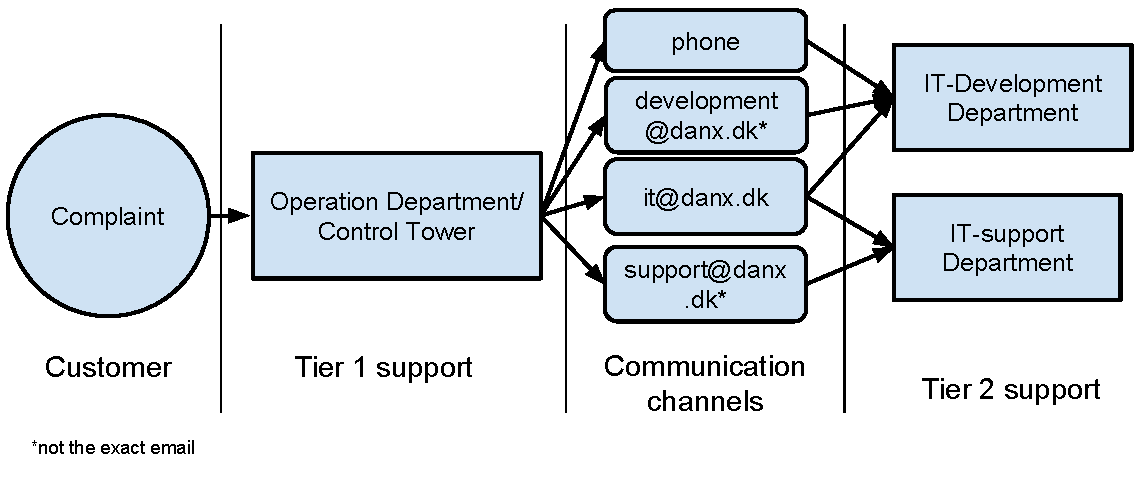
\includegraphics[scale=0.8]{img/Work_Practice_Flow}

\subsection{Stakeholder Analysis}
The purpose of the stakeholder analysis is to map the general interests of the key players with their role in the project.

\vspace{3mm}
\begin{tabular}{ | p{2.4cm} || p{5.9cm} | p{5.9cm} | }
\hline
\rowcolor{GR}
\textbf{Stakeholder} & \textbf{General interests} & \textbf{Key interests and role in relation to the project}\\ \hline \hline
Operations department & Ensure that the delivery of spare parts is unhindered, by coordinating and integrating. & Providing effective customer support.\cite{gert016} Possibly part of the solution, because employees have knowledge of customer support. \\ \hline
Gert Philipsen & Ensuring that the operational department is functional and optimizing it. & Optimizing the operational department.\cite{gert015} As he leads the operational department his opinion on the project is important \\ \hline
Lasse Trier & On-time delivery of customer integrations and customer support & Lasse would like to document what customer support he has provided.\cite{lasse007}\\\hline
\end{tabular}

\section{Goals, Problems and Needs}
\label{sec:goalsproblemsandneeds}
This section describes the most significant goals and the problems that can hinder reaching the goals of the selected departments, or the goals described in chapter~\ref{chap:strategicalignmentreport}.
\subsection{Goals}
The IT department and the operational department has to integrate customers before their old contract expires. This can be everything between 1 day and to the 1st of next month.\cite{gert013}\cite{lasse008} It is important that the IT solution is ready on time, as DANX will not wait for the IT solution before they start working with the client\cite{lasse008}, this is to uphold the high service level. This means that if a system is not ready on time, DANX will start working with the customer without the IT system.\\
Not having an IT system results in additional workload because the data that the system creates and maintains automatically needs to be done manually. Fast integration is an important goal for the company because it makes the company fast in comparison to the competitors, some of which uses approximately 14 days for the integration. For reference see section~\ref{sub:competitor_analysis}\\
An important factor that makes DANX competitive, and therefore can be perceived as a goal, is that the customer can contact the IT department directly by email or phone avoiding the communication chain starting from the control tower. The problems that some customers of DANX experience can have serious consequences for their production or other practices that are hindered by the lack of a spare part.\cite{gert018} Having a shorter chain of communication and therefore a shorter response time can be a valuable service.\cite{lasse012}\\
These goals puts variable work pressure on the employees of the development department, because integration is a task that has to be done one time per customer, but takes at least an entire day. Customer problems are also varying.

\subsection{Problems}
There are several problems that can hinder the work practices that allows these goals to be reached. If the customer’s IT department is not ready on time, the integration can not be completed and DANX is forced to work without an IT system.\cite{lasse008}\\
In some cases the submitter of a customer problem is not clearly visible from the email containing the problem description. In this case the IT department spends from 10 to 15 minutes\cite{lasse013} on clarifying who the submitter of the problem is.\\
The IT support and IT development department spent time on reading mails that should be mailed to the other department because they share it@danx.dk.\cite{lasse010}\\
Internal support requests takes longer time to solve because of lacking information. The lacking information is retrieved by additional emails or phone contact.\\
The operational manager, can not supervise which customer support requests that are done and how long time it is pending. With this lack of knowledge it is complicated to optimize customer support. In the current situation, the knowledge of a specific problem can only be obtained by examining emails or talking to the employees that are responsible for solving the problem. The responsibility assignments are not documented, which complicates this further.\cite{gert012} The operational manager can not guarantee that a problem is solved within a given time period with no knowledge of the responsibility assignments.\\
With no documentation of customer support, KPIs of customer response time can not be established.\cite{gert011} The bigger DANX grow, the harder it is for a single manager to maintain an overview of how well the customer support is doing. As one of the goals of DANX is to grow, this issue becomes increasingly relevant.

\subsection{Needs}
The needs of the department is based on their current work practice, problems and the strategies identified in the Strategic Alignment Report.\\
The most important requirement for a solution to a problem within DANX is that it supports their rapid growth, because it is a business goal.\\
The SWOT analysis revealed that DANX has an advantages in direct customer support and fast integration, which the solution must keep or strengthen.\\
To keep the direct customer support, the solution can not change the way that customers contacts and communicate with DANX.\\
The IT development department has potential for optimization of work practices. A lot of the work that is done is information gathering that is necessary because the submitter of a problem has not included enough information, both for internal and external problems.\cite{lasse010}\\
As this increases the workload for the problem solver, providing this missing information can save time.\\
The solver of external problems is primary Lasse, and as he is responsible for much of the integration, support and prioritization of work, reducing his workload is a need. As DANX grows his workload will grow, because it is assumed that increasing the number of customers increases the number of support requests.\\
Both the IT development department and the operational department needs documentation of customer support in order to have data to base evaluation on. With no evaluation the operational manager can not know how well customer support is doing, and has no way to know where to optimize the department.\\
It is assumed that growth introduces additional employees and it is harder to asses an increasing number of employees’ performance without documentation. To guarantee that customer support requests are answered on-time, documentation that keep track of the request and the responsible employee is needed. It is assumed that an increasing amount of employees makes the need for employee evaluation increasingly important.

\subsection{Parallel projects}
The operation of DANX is educating their staff to understand the responsibilities of the different IT departments, such that they can submit the problem to the correct department, avoiding the responsibility overlap of it@danx.dk. In the future, the employees will preferable use the department-specific email, possibly decreasing the time that both departments uses on considering the problem.\cite{gert017}

\section{Ideas for solutions and suggested priorities}
\label{sec:ideas}
When trying to specify a solution it is important to be aware of what aspect of the problem that specific solution benefits, as a problem might require several solutions in order to be fixed.\\
Our focus is to provide DANX with means to generate documentation in a fast, efficient and uniform way, ultimately strengthening DANXs position in regards to keeping a high degree of service towards customers.\\

\subsubsection{First proposal}
Our first proposal is a simple software system with three main functions.\\
First it enables end-users(DANX employees) to keep track of support requests.\\
A request should contain information about the customer, description of the problem, the DANX employee handling the requests, the timestamps for when it was received, and when it was resolved.\\
Second it provides end-users with a filtering option to make sure that the data can be reviewed in an understandable fashion.\\
Third, since some support requests feature emails, it features a way to attach these to the requests.\\
This will give DANX documentation of how much support the IT-development department provides and how much the operations department provides, as well as the time spent providing it.\\
The time factor is a great addition, as this can be used to determine response times, and management is able to create KPIs eg. response time should be no greater than certain amount of days.\\
Furthermore the function of following up on unresolved tickets is a great tool for improving customer satisfaction.\\

\subsubsection{Second proposal}
The second proposal is in continuation of the first proposal.\\
It is similar to the first proposed system but it should additionally contain some extended information on the requests, particularly solutions to the problems and labels.\\
The labels should provide a means to group solutions into which types of problems they are.\\
An example of this could be the labels ‘EDI integration’ or ‘TrackIT integration’, providing end-users with a way to group possible solutions when providing support in certain fields.\\
When applying the second solution multiple benefits are achieved.\\
First and foremost, a well documented issue, which frequently occurs, might have a general solution for multiple customers, ultimately saving time spent on contacting experts within that particular field. \\
Secondly it might illustrate a flaw in the current practices, and the documented pattern can then be used to pinpoint the exact reason for the occurrence, which would make it easy for the experts to correct the issue or proactively attempt to avoid it.\\
In the second solution a crucial factor to success would be the fact that end-users of the system are provided with training in using the system and identifying problem types.\\
This is to ensure that they have the qualifications to tag the requests with their respective labelling.\\
This is important since the system would not function efficiently in regards to filtering if everything is mislabeled.\\
A downside to the second solution is that it will affect the time spent on initially handling the requests, seeing the employee has to manually write it into the system.\\
If an email has been sent it is possible to associate it with the request and save some time, but nevertheless one has to create the request.\\
When working with both solutions the parties affected directly would be the operations department and the IT development department.\\
This is due to the fact that these departments have first-hand contact with customers and are solving the customers problems.\\

\subsubsection{Customer impact}
Another important thing is that the systems are not to be forced upon the customers of DANX, as this might seem as a reduction in quality for them.\\
The system is intended to alter the workflow for the people answering the calls and the people handling the requests, and provide a structured way to review the work of the affected departments.\\
As Gert Phillipsen has expressed its important that solutions to problems are a part of the new system and hence we would recommend the second solution to have a higher priority.\cite{gert003}

